\section{Virtueel geheugen}

\subsection{Hardware en besturingsstructuren}

Belangrijkste punten in het geheugenbeheer:

\begin{itemize}
\item Verwijzingen naar het geheugen zijn logische adressen die dynamisch worden vertaald naar fysische adressen at run time. Een proces moet in en uit geswapd worden uit het hoofdgeheugen tijdens uitvoering, waardoor het kan zijn dat het verspreid wordt over verschillende plaatsen in het geheugen.
\item Een proces kan gesplitst worden in stukken, deze moeten niet opeenvolgend opgeslagen worden in het hoofdgeheugen.
\end{itemize}

Doorbraak in het geheugenbeheer:

Als beiden bovenstaande kenmerken aanwezig zijn, dan is het niet nodig dat alle pagina’s of alle segmenten van het proces zich in het hoofdgeheugen vinden tijdens uitvoering. Zolang dat de volgende datalocatie en de volgende instructie zich in het geheugen bevinden kan de uitvoering toch nog zeker doorgaan.

Uitvoering van een proces:

\begin{itemize}
\item Besturingssysteem steekt delen van het programma in het hoofdgeheugen.
\item De residente set is de verzameling van processen die zich in het hoofdgeheugen bevinden.
\item Een interrupt wordt gegeven wanneer een adres nodig is dat niet in het hoofdgeheugen bevindt.
\item Het besturingssysteem plaatst het proces in een geblokkeerde toestand. 
\end{itemize}

Inlezen van een proces:
\begin{itemize}
\item Besturingssysteem doet een disk I/O Lees aanvraag.
\item Een ander proces wordt geactiveerd om uit te voeren terwijl de I/O-operatie wordt uitgevoerd.
\item Een interrupt wordt gegeven wanneer de disk I/O compleet is, het betrokken proces wordt in de ready state gezet.
\end{itemize}
	
Gevolgen van deze nieuwe aanpak:

\begin{itemize}
\item Meer processen kunnen zich bevinden in het hoofdgeheugen. Als er zoveel processen in het hoofdgeheugen zijn, dan is de kans zeer groot dat zich er een proces in de ready toestand bevindt op elk moment.
\item Een proces kan groter zijn dan het totale hoofdgeheugen. 
\end{itemize}

Er zijn twee soorten geheugen:

\begin{itemize}
\item reële geheugen (de plaats waar processen uitgevoerd worden)
\item virtuele geheugen (de ruimte die wordt toegewezen op schijf)
\end{itemize}

\subsubsection{Lokaliteit en virtueel geheugen}

Trashing: wanneer de processor meer bezig is met het in en uitswappen van processen dan met de uitvoering ervan. Dit gebeurt wanneer het reële geheugen overvol zit en er continu processen moeten uitgeswapt worden om plaats te maken voor andere stukken van een proces. Wanneer een uitgeswapt deel echter meteen weer nodig is, dan moet dit worden ingeswapt. Veel swappen dus en weinig uitvoer.

Trashing is te voorkomen door te voorspellen welke delen van een proces in de nabije toekomst zullen nodig zijn op basis van het recente verleden.

Dit is gebaseerd op het lokaliteitsbeginsel.

Het lokaliteitsbeginsel verwijzingen naar programma's en gegevens van processen hebben de neiging op te hopen tot een cluster => het is geldig om te veronderstellen dat slechts een deel van een proces nodig is voor een beperkte tijd => het is mogelijk om een voorspelling te maken van de stukken die zullen nodig zijn in de nabije toekomst wat trashing voorkomt.

=> virtueel geheugen kan werken aangezien er een voorspelling kan gemaakt worden en trashing kan voorkomen worden, anders was het maar een slecht idee aangezien het na verloop van tijd aanleiding zou geven tot trashing

\textbf{Wat nodig voor virtueel geheugen:}

\begin{itemize}
\item Hardwareondersteuning: toepassen paginering en segmentering + vertaling van adressen
\item Softwareondersteuning: beheren van de verplaatsing van delen proces tussen hoofd-en secundair geheugen
\end{itemize}

\subsubsection{Pagineren}

Elk proces heeft zijn eigen pagetable, elke page table entry bevat het frame nummer van de overeenkomstige pagina in het hoofdgeheugen.

Twee extra bits zijn nodig om te bepalen welke pagina zich in het hoofdgeheugen bevindt en welke niet(de p-bit) én ook om te bepalen welke inhoud van de pagina veranderd is sinds het geladen werd (de m-bit).

\begin{figure}[htp]
    \centering
            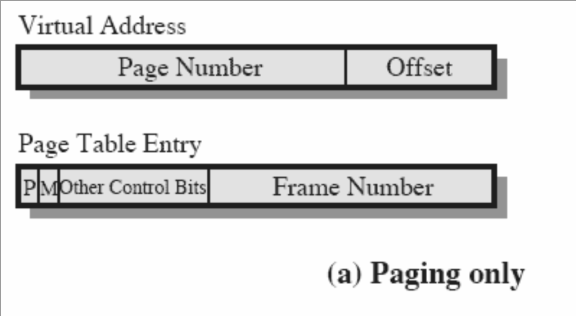
\includegraphics[width=4in]{img/pagineren.png}
        \caption{Paging only}
    \label{fig:Paging only}
\end{figure}

Paginatabelstructuur

\begin{itemize}
\item Lezen van een woord uit het geheugen: vertalen van een virtueel (logisch) adres(paginanummer en offset) in een fysiek adres(framenummer en offset).
\item Paginatabel heeft variabele grootte (afhankelijk van grootte proces) => niet opslaan in registers maar in hoofdgeheugen.
\item (zie fig. 8-3) proces wordt uitgevoerd => register bevat beginadres van de paginatabel van het proces
\item Het paginanummer wordt gebruikt als index in de tabel om het bijhorende framenummer op te zoeken.
\item Reëel adres = framenummer + offset
\end{itemize}

\begin{figure}[htp]
    \centering
            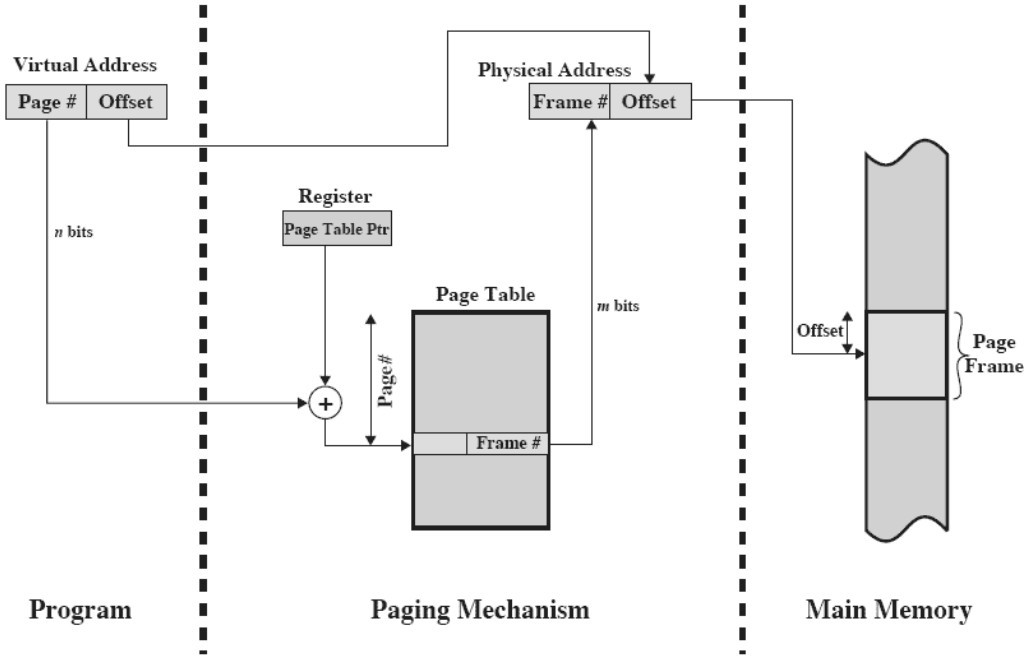
\includegraphics[width=4in]{img/paginatabelstructuur.jpg}
        \caption{paginatabelstructuur}
    \label{fig:paginatabelstructuur}
\end{figure}

De meeste systemen gebruiken 1 paginatabel per proces <-> VAX: ieder proces kan 231 (2 G) groot zijn. Stel: paginagrootte: 512 byte => 222 PTE's => Paginatabel = enorm => paginatabel wordt ook ingedeeld in pagina's en wordt opgeslaan in virtueel geheugen. => wordt een proces uitgevoerd, dan moet er een deel van de paginatabel in het hoofdgeheugen staan en al zeker de PTE van de huidige pagina.

Sommige systemen gebruiken een systeem met twee niveaus: bevat een paginadirectory (elke ingang van deze directory verwijst naar een paginatabel). Is de lengte van het paginaoverzicht X en is de lengte van de paginatabel Y, dan bestaat een proces uit X*Y pagina's

Stel:

\begin{itemize}
\item adressen van 32 bits
\item paginagrootte: 212 (KB) => virtueel geheugen van 232 bytes (4GB) kan 22 0 aantal pagina’s bevatten
\item iedere PTE = 4B => de volledige paginatabelgrootte = 220 * 4 = 222 bytes(4MB)
\item mogelijkheid om een gebruikerspaginatabel van 210 pagina's in het virtueel geheugen te hebben en bereikbaar te maken a.d.h.v. een basispaginatabel met 210 PTE's en een grootte van 212 (4 KB) in het hoofdgeheugen. De basispaginatabel blijft altijd in het hoofdgeheugen!
\item 
\item 
\end{itemize}

Adresvertaling bij een systeem met twee niveaus:

\begin{itemize}
\item eerste 10 bits van virtuele adres = index in de basispaginatabel om de PTE te verkrijgen voor een pagina in de gebruikerspaginatabel(paginafout: refereren naar een pagina die niet aanwezig is in hoofdgeheugen).
\item Is de pagina wel aanwezig in het hoofdgeheugen, dan zijn de volgende 10 bits in het adres de index in de gebruikersPTE-pagina om de PTE te vinden van de pagina waarnaar verwezen wordt in het virtuele adres
\end{itemize}

\begin{figure}[htp]
    \centering
            \includegraphics[width=4in]{img/}
        \caption{}
    \label{fig:}
\end{figure}

\textbf{Geinventeerde paginatabel}

Nadeel van hogergenoemde paginatabellen is dat de grootte ervan evenredig is met de omvang van de virtuele adresruimte.

Bij een ander type paginatabel is dit niet, hierbij wordt er gewerkt met een geïnverteerde paginatabelstructuur (indexeert de items op framenummer i.p.v. op virtueel paginanummer) waarbij het paginanummer (onderdeel van virtueel adres) gehashed wordt en deze hash verwijst naar de geïnverteerde paginatabel. Deze tabel heeft een vaste grootte, namelijk als een fysiek geheugen 2m   frames bevat dan is er plaats in de tabel voor 2m items waarbij item z verwijst naar frame i.

De geïnverteerde paginatabel bevat 1 item voor elke werkelijke frame i.p.v. 1 item per virtuele pagina.

Collision (de hashes van twee verschillende paginanummers zijn gelijk) is mogelijk => er wordt gewerkt met een kettingtechniek om toch tot het juiste adres te komen.

Ieder item in de geïnverteerde paginatabel bevat volgende gegevens:


\begin{itemize}
\item Paginanummer: (paginanummer virtueel adres)
\item PID: proces dat deze pagina in bezit heeft (combinatie paginanummer-PID is uniek => kan gebruikt worden als er collision is bij hashing)
\item Besturingsbits: bvb.: modified, referenced, valid, beveiligings- en vergrendelingsinfo
\item Kettingpointer: is 0 als er geen koppelingen zijn met andere pagina's. bevat een nummer van 2m-1 dat het rangnummer is in de tabel van het volgende item in de ketting
\end{itemize}

\begin{figure}[htp]
    \centering
            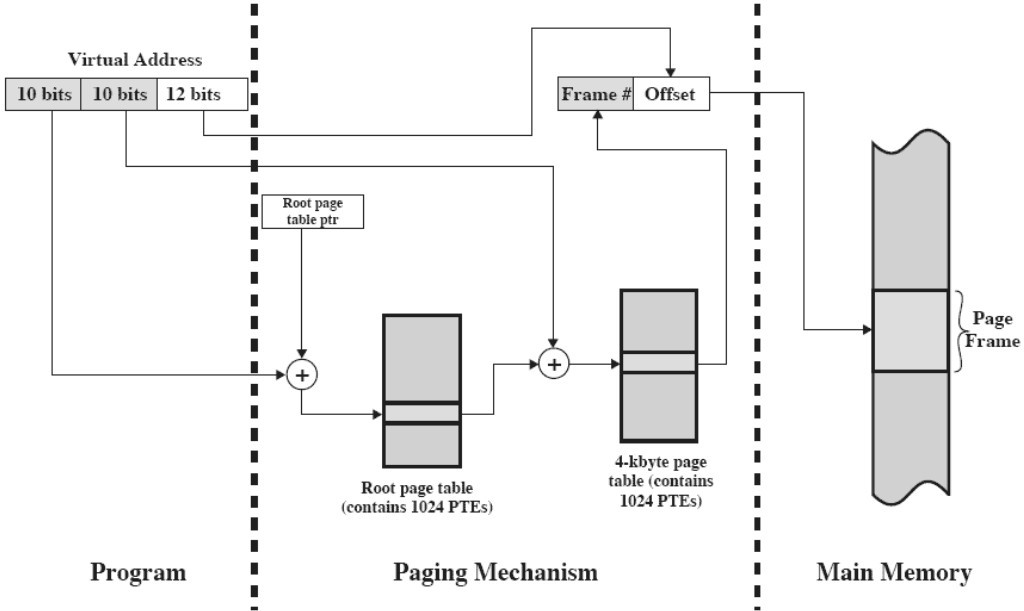
\includegraphics[width=4in]{img/Geinventeerdepaginatabel.jpg}
        \caption{}
    \label{fig:}
\end{figure}

\textbf{Translation lookaside buffer}

Elke virtuele verwijzing naar het virtuele geheugen kan twee fysieke geheugen verwijzingen zijn:

\begin{itemize}
\item ophalen van gegevens
\item ophalen van de juiste PTE
\end{itemize}

Als beiden moeten gebeuren tgv dezelfde verwijzing, dan moet er eerst gezocht worden naar de juiste PTE (PageTableEntry) én dan nog eens naar de juiste gegevens op de schijf => verdubbeling van geheugen- toegangstijd.

Dit wordt opgelost door TLB (Translation Lookaside Buffer) = speciale cache voor paginatabelingangen; bevat de PTE's die recent het meest gebruikt zijn.

Werking:

\begin{enumerate}
    \item processor ontvangt een virtueel adres
    \item is de gewenste PTE in de TLB, dan wordt het framenummer opgevraagd en wordt het reële adres gevormd, samen met de offset
    \item TLB-miss => met paginanummer als index kijken of de 'present' bit van de pagine in de PTE in de paginatabel op 1 staat
        \begin{enumerate}
        \item Bit staat op 1: pagina staat in het hoofdgeheugen => het framenummer wordt opgevraagd uit de PTE en het reële adres wordt gevormd + de TLB wordt bijgewerkt door deze nieuwe PTE toe te voegen.
        \item Bit staat op 0: paginafout en dan verlaten we de hardware om het OS de pagina re laten laden en om de paginatabel bij te werken.
        \end{enumerate}
\end{enumerate}

Opmerking bij onderstaande figuur: wanneer I/O bewerking gebeurt, voert processor ondertussen ander proces(sen) uit.

Overeenkomstig het beginsel van lokaliteit: de meeste verwijzingen naar virtueel geheugen zijn verwijzingen naar locaties in recent gebruikte pagina's.

Het opzoeken in de TLB gaat sneller dan het opzoeken in de paginatabel omdat het gaat om cachegeheugen!

\begin{figure}[htp]
    \centering
            \includegraphics[width=4in]{img/}
        \caption{}
    \label{fig:}
\end{figure}


\begin{figure}[htp]
    \centering
            \includegraphics[width=4in]{img/}
        \caption{}
    \label{fig:}
\end{figure}

Associatieve vertaling (associative mapping): de hardware is in staat om verschillende TLB entries tegelijkertijd te doorzoeken (daarom is het nodig dat iedere TLB ingang naast het paginanummer ook de volledige PTE bevat)

Directe vertaling wordt gebruikt om op te zoeken in de paginatabel.

\begin{figure}[htp]
    \centering
            \includegraphics[width=4in]{img/}
        \caption{}
    \label{fig:}
\end{figure}

Het gebruik van een TLB vereist interactie met de hoofdgeheugencache. Stel dat de PTE zich in de TLB bevond of in de paginatabel na een TLB-miss, dan wordt het reëel adres gevormd. Dan wordt er in de hoofdgeheugencache nagekeken of het blok met het vereiste woord zich daarin bevindt. Is dat niet zo, dan moet de processor het inladen uit het hoofdgeheugen.

\textbf{Paginagrootte}

Hoe kleiner een pagina des te kleiner is de interne fragmentatie MAAR des te groter is het aantal pagina's dat het proces nodig heeft (dus ook meer pagina's die moeten aanwezig zijn en hoe groter de page tables).

De meeste apparaten voor secundaire opslag vereisen echter een grotere paginagrootte voor een meer efficiënte blokoverdracht van gegevens (daarvoor dienen ze, om grote hoeveelheden aaneengesloten data te verwerken).

Nog iets om mee rekening te houden is de invloed die de paginagrootte heeft met betrekking tot paginafouten:

\begin{itemize}
\item paginagrootte klein $\Rightarrow$ weinig paginafouten want er kunnen veel pagina's worden ingeladen in het hoofdgeheugen.
\item Beginsel van lokaliteit: na verloop van tijd bevinden zich in het geheugen alle gedeelten van het programma in de buurt van frequente verwijzingen.
\item als de grootte toeneemt, bevat elke afzonderlijke pagina locaties die zich verder dan een recente verwijzing bevinden => invloed beginsel lokaliteit neemt af en dan stijgt de foutfrequentie
\item naarmate de pagina's nog groter worden zullen ze groot genoeg worden om ganse processen te bevatten waardoor er geen paginafouten meer optreden
\end{itemize}

\begin{figure}[htp]
    \centering
            \includegraphics[width=4in]{img/}
        \caption{}
    \label{fig:}
\end{figure}

De foutfrequentie is ook afhankelijk van het aantal frames die worden toegewezen aan een proces. Naarmate het aantal toegewezen frames stijgt, daalt het aantal paginafouten. Het ontwerp van de paginagrootte hangt ook samen met de grootte van het fysieke hoofdgeheugen en van het programma. Naarmate het geheugen groter wordt, groeit ook de adresruimte die door toepassingen kan worden gebruikt. De invloed van het beginsel van lokaliteit - - op moderne programmeertechnieken:

OO-programmeren: verwijzingen worden op korte tijd sterk verspreid over een groot aantal objecten. Multithreading: abrupte veranderingen in de instructiestroom en tot verspreide geheugenverwijzingen

Probleem: als lokaliteit afneemt, dan neemt het aantal hits in de TLB ook af en vormt het opzoeken in de TLB een bottleneck.

\textbf{Hoe dit oplossen?}

\begin{itemize}
\item Grotere TLB kan maar zal minder wsl zijn
\item Grotere pagina's => iedere TLB ingang verwijst naar een groter stuk geheugen (maar het vergroten van de grootte kan leiden tot een vermindering aan prestaties)
\end{itemize}

Er is geëxperimenteerd geweest met meerdere paginagrootten waardoor er een flexibiliteit ontstaat die toelaat de TLB efficiënt te gebruiken.

\subsubsection{Segmenteren}

\textbf{Segmenteren} staat toe dat de programmeur het geheugen ziet als meerdere adresruimtes of segmenten.

\textbf{Gevolgen voor het virtueel geheugen:}

\begin{itemize}
\item Kan oneven zijn, een dynamische grootte.
\item Vereenvoudigt het werken met groeiende gegevensstructuren.
\item Staat toe dat programma’s onafhankelijk gewijzigd en gehercompileerd kunnen worden.
\item Segmentatie is geschikt voor het delen van data tussen processen.
\item Segmentatie is geschikt voor bescherming.
\end{itemize}

\textbf{Organisatie}

Elk proces heeft een eigen segmenttabel. Elke segmenttabelingang bevat het beginadres van het bijhorende segment. Elke entry bevat ook de lengte van het segment.

Een bit is nodig om te bepalen of het segment zich al in het hoofdgeheugen bevindt.

Een andere bit is nodig om te bepalen of het segment gewijzigd is sinds het werd ingeladen in het hoofdgeheugen.


\begin{figure}[htp]
    \centering
            \includegraphics[width=4in]{img/}
        \caption{}
    \label{fig:}
\end{figure}

Basismechanisme voor lezen van een woord uit het geheugen: vertalen van een virtueel adres(segmentnummer en offset) naar een reëel adres m.b.v. de segmenttabel:

\textbf{Een register bevat het beginadres van de segmenttabel, segmentnummer in virtueel adres dient als index voor de juist STE in de tabel. De STE geeft dan weer aan wat het basisadres is van het segment in het hoofdgeheugen. Dat basisadres + offset = reëel adres.}


\subsubsection{Gecombineerd pagineren en segmenteren}

Pagineren is transparant voor de programmeur en elimineert externe fragmentatie en zorgt daarmee voor een efficiënt gebruik van het hoofdgeheugen. Segmentatie is zichtbaar voor de gebruiker en heeft de mogelijkheid van werken met groeiende gegevensstructuren, modulariteit en de ondersteuning van delen en bescherming. Elk segment wordt opgedeeld in een pagina’s van vaste grootte.

\begin{figure}[htp]
    \centering
            \includegraphics[width=4in]{img/}
        \caption{}
    \label{fig:}
\end{figure}


\subsubsection{Bescherming en delen}

Bescherming: elke STE: een lengte en basisadres => een programma kan geen toegang krijgen buiten de grenzen van een segment.

Deling: er kan naar een segment verwezen worden in de segmenttabellen van meerdere 
processen. Dit kan ook in een pagineringssysteem maar dan is het onzichtbaar voor de programmeur.


\begin{figure}[htp]
    \centering
            \includegraphics[width=4in]{img/}
        \caption{}
    \label{fig:}
\end{figure}
